% vim:spelllang=uk,en
\documentclass{diploma}

\usepackage{amsmath}
\usepackage{cmap}
\usepackage{cite}
\pdfcompresslevel=9 % сжимать PDF
\usepackage{pdflscape} % для возможности альбомного размещения некоторых страниц
\usepackage{moreverb}
\usepackage{multirow}
\usepackage{misccorr}

\usepackage{relsize}
\usepackage{listings}
\lstset{breakatwhitespace=false
       ,breaklines=true
       ,commentstyle=\rm
       ,escapeinside={\%*}{*)}
       ,frame=none
       ,language=Matlab
       ,stringstyle=\rm
       ,title=\lstname
       }
\titleformat{\chapter}[hang] % указуємо, що модифікуємо саме розділ
      {\centering\bfseries\MakeUppercase} % указуємо формат назви (жирний, "усі великі")
      {\hspace{1cm}\thechapter} % указуємо формат власне номера: це буде просто число, без крапки
      {0.5em} % відстань між номером і назвою
      {} % текст, що передує назві
% займемося розділами
      % \usepackage{xcolor}}
      % \usepackage{tikz}

% \newcommand{\mycbox}[1]{\tikz{\path[draw=#1,fill=#1] (0,0) rectangle (1em,1em);}}
% \renewcommand{\cftchapaftersnum}{\!\!\small\tikz{\path[draw=white,fill=white] (0,0) rectangle (1em,1em);}}% adds dot after chapter title in ToC
\makeatletter
  \renewcommand{\thechapter}{\arabic{chapter}}
\makeatother
\begin{document}
\chapter*{АНОТАЦІЯ}
  \thispagestyle{empty}
  Ця дипломна робота присвячена проектуванню та розробці системи відновлення
  спотворених зображень, що використовує деконволюцію (обернену згортку) як
  інструмент для відновлення зображення та перетворення Фур’є як інструмент
  для отримання його частотної характеристики.

  У рамках цієї роботи був проведений аналіз існуючих рішень для відновлення
  зображень, та обраний оптимальний метод, а також існуючи методи отримання
  початкового наближення функції розподілу точки/

  В програмній реалізації були використані наступні методи: перетворення
  Фур’є, обернене перетворення Фур’є.

  Робота складається зі вступу, 5 розділів та висновків, і налічує 77
  сторінок.
  Містить 46 ілюстративних матеріалів, 1 таблиці, 2 додатки та посилається на
  14 літературних джерел.

  Ключові слова: зображення, розмиття, згортка, конволюція, деконволюція,
  перетворення Фур’є, функція розподілу точки, артефакти, відновленн.
  \clearpage
\chapter*{ABSTRACT}
  \thispagestyle{empty}
  This diploma thesis deals with the development of mathematical system for
  restoring blurred images using deconvolution and Fourier transformation.

  The comparative analysis of existing algorithms for restoring quality of
  blurred images is fulfilled and discussed.
  Among it methods of estimating point spread function are also discussed.

  In the software realisation were used such techniques, as Fourier
  transform, inverse Fourier transform, object"=oriented programming.

  Thesis consists of introduction, 5 chapters and conclusion.
  It has 77 pages, 46 figures, one table, two appends and has links to 14
  bibliographical items.

  Keywords: image, blurring, convolution, deconvolution, Fourier transform,
  point spread function, restoring
  \clearpage
\maketitlepage
\shortings
FFTW --- Fastest Fourier Transform in the West\\
\noindent
FT --- Fourier Transform\\
\noindent
GPL --- The GNU General Public License\\
\noindent
JPEG --- Joint Photographic Experts Group\\
\noindent
PNG --- Portable Network Graphics\\
\noindent
PSF --- Point spread function\\
\noindent
АЦП --- Аналого"=цифровий перетворювач\\
\noindent
ВВ --- Вогнегасник вуглекислотний\\
\noindent
ВДТ --- Відеотермінал\\
\noindent
ПЕОМ --- Персонально Електроно"=Обчислювальна Машина
\clearpage
\intro
  Сьогодні цифрові зображення набули значної популярності.
  Цифрові фотокамери є в більшості мобільних телефонах, ноутбуках та в іншій
  портативній техніці (не кажучи про власне фотоапарати).

  Одна з умов, що забезпечили таке поширення цієї техніки було те, що люди
  бажають зафіксувати на цифровому знімку якусь подію якнайшвидше.
  Зараз досить достати пристрій, натиснути кнопку й почати знімати.

  Одним з недоліків такого методу є те, що такі фотографії часто бувають
  не в фокусі або розмитті.
  Дуже часто немає нагоди перезняти такі невдалі кадри.

  Відновлення спотворених зображень є одною з найцікавіших й важливих проблем
  обробки зображень --- як з теоретичної, так і з практичної точок зору.
  Окремими випадками є розмиття через неправильний фокус та змазування --- ці
  дефекти знайомі майже усім, хто хоч раз користувався фотокамерами.
  Відновлення зображень з цими дефектами --- дуже складна задача.

  Багато людей вважає, що розмиття --- необоротна операція й інформація
  безповоротно втрачається, адже ж кожний піксель перетворюється на пляму, все
  змішується, а при великому радіусі розмиття так і зовсім отримуємо
  однорідний колір по всьому зображенню.
  Але насправді вся інформація просто перерозподіляється по деякому закону та
  може бути однозначно відновлена за деякими обмеженнями.
  Виняток становлять лише границі зображення шириною в радіус розмиття.

  Результат значно погіршується якщо додати у зображення шум.
  Але кожне реальне зображення містить у собі певну кількість шуму, тому
  алгоритми повинні враховувати цей факт.

  Існують багато методів відновлення зображень, що дозволяють прибрати брак з
  фотографії.
  Одним з таких методів є операція зворотної згортки, або деконволюції, яка
  буде розглянута в цій роботі.
  \clearpage
\chapter{ПОСТАНОВКА ЗАДАЧІ}
\pagestyle{plain}
  Необхідно розглянуті теоретичну основу відновлення зображення за допомогою
  деконволюції.

  Зробити порівняльний аналіз методів відновлення зображень за відомою
  функцією розподілу точки.
  Для цього необхідно змоделювати певне спотворення, яке б було близьким до
  реального (включаючи шум), й відновити отримане зображення.
  Порівняти результати.

  Дослідити області застосувань методів відновлення зображень в залежності від
  різних видів розмиття або змазування.
  Для цього необхідно порівняти результати відновлення зображень, що були
  спотворені найпоширенішими функціями розподілу точки.
  Порівнювати слід за наявністю артефактів, шуму, загальної якості
  відновленого зображення.

  Дослідити можливість отримання наближення функції розподілу точки за
  заданим, розмитим зображенням.
  Потрібно описати методики й приблизний алгоритм, який би дозволяв отримувати
  гарне наближення до функції розподілу точки.
  \clearpage

\chapter{ТЕОРЕТИЧНІ ВІДОМОСТІ}
  \section{Модель процесу спотворення}
    Сигнал --- зміна фізичної величини (наприклад, температури, тиску
    повітря, світлового потоку, сили струму тощо), що використовується для
    пересилання даних.
    Сигнали можуть бути:
    \begin{itemize}
      \item Одновимірними: інфрачервоні спектри або звукові сигнали.
      \item Двовимірними: цифрові зображення.
      \item Тривимірні: зображення, отримані мікроскопом (так звані Z"=стеки).
      \item Багатовимірні: серії трьохвимірних сигналів, зняті у послідовні
        моменти часу.
    \end{itemize}

    Будемо розглядати напівтонові чорно"=білі зображення (вважатимемо, що для
    обробки повнокольорового зображення досить повторити всі необхідні кроки
    для кожного з колірних каналів).
    Введемо наступні позначення:
    \begin{itemize}
      \item $x, y$ --- координати пікселю на зображенні (горизонтальна та
        вертикальна).
      \item $f\left( x, y \right)$ --- вихідне неспотворене зображення.
      \item $h\left( x, y \right)$ --- функція ,,спотворення''.
      \item $n\left( x, y \right)$ --- адитивний шум.
      \item $g\left( x, y \right)$ --- результат спотворення, тобто те, що ми
        спостерігаємо в результаті (зміщене або розмите зображення).
    \end{itemize}

    Саму модель процесу спотворення можна представити у вигляді наступного
    рівняння:
    \begin{equation}
      g\left( x, y \right) = h\left( x, y \right) \ast f\left( x, y \right) +
      n\left( x, y \right)
      \label{eq:model}
    \end{equation}

    Задача відновлення спотвореного зображення полягає в знаходженні
    найкращого наближення $f^\prime$ вихідного зображення.

    Згортка --- операція, що показує ,,схожість'' однієї функції з
    відбитою та зрушеною копією іншої.
    В математиці, згортка --- це математична операція двох функцій $f\left(
    x \right)$ і $g\left( x \right)$, що породжує третю функцію, яка зазвичай
    може розглядатися як модифікована версія однієї з початкових.
    По суті, це особливий вид інтегрального перетворення:
    \begin{equation}
      \left( f * g \right)\left( x \right) \stackrel{\mathrm{def}}{=}\
      \int_{-\infty}^\infty f(\tau)\, g(t - \tau)\, d\tau
      \label{eq:convolution-definition}
    \end{equation}

    Через операцію згортки описуються багато деградацій, що зустрічаються на
    практиці:
    \begin{itemize}
      \item не сфокусованого розмиття;
      \item розмитість (наприклад, через струс камери);
      \item дифракційного розмиття;
      \item тощо.
    \end{itemize}
    \clearpage
    \subsection{Функція спотворення}
      В процесі спотворення кожен піксель початкового зображення
      перетворюється в пляму при розмитті та у відрізок у випадку
      простого змазування.
      Власне кажучи, згортка --- це процес, що певним чином ,,змішує'' два
      сигнали.
      Або, навпаки, можна сказати, що кожен піксель зображення, що було
      спотворене, ,,збирається'' з пікселей певного околу початкового
      зображення.

      Кожна точка першого сигналу (назвемо його $f\left( x, y\right)$)
      перероблюється у копію другого сигналу (назвемо його $h\left( x, y
      \right)$).
      Кожна така копія має таку загальну інтенсивність, що дорівнює
      інтенсивності початкової точки сигналу $f\left( x, y \right)$.
      Усі ці копії накладаються одна на одну, отримуючи таким чином сигнал
      $g\left( x, y \right)$, що є згорткою сигналів $f\left( x, y \right)$ та
      $h\left( x, y \right)$.

      \begin{figure}[!htp]
        \centering
        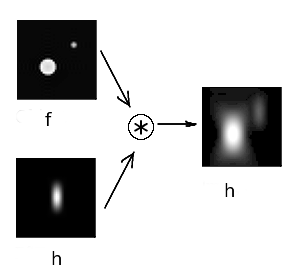
\includegraphics{conv.png}
        \caption{Приклад згортки}
        \label{fig:example-convolution}
      \end{figure}

      Саме функція спотворення й показує, по якому закону ,,збирається'' або
      розмазується пікселі зображення.
      Функція спотворення також відома як функція розподілу точки (англ.~PSF
      --- Point spread function), ядро (англ.~kernel) оператору спотворення,
      адже вона визначає, як саме кожна точка сигналу $f$ ,,розсіюється '' в
      копію PSF.
      Розмірність цієї функції, як правило, менше за розмірність самого
      зображення.

      Саме тому операція згортки також відома як суперпозіціонний інтеграл, а
      обернена операція --- розділенням сигналів.
      Але згортка є комутативною операцією --- ми можемо визначити сигнал $f$
      як PSF для сигналу $h$:
      \[ f * h = h * f \]

      Дуже багато деградацій, що зустрічаються повсякденно, можуть бути
      описаними за допомогою однієї й тієї ж самої операції.

      В вищенаведеному описі операції згортки було допущено, що однакова PSF
      була застосована до всіх точок сигналу $f$.
      Це припущення має місце в багатьох теоретичних викладках і має назву
      згортки з інваріантною у просторі функцією розсіювання точки.
      Але в реальних ситуаціях має місце зміна (найчастіше поступова) PSF з
      переміщенням по сигналу $f$.
      Такий випадок називається згорткою зі змінною у просторі PSF.
      В таких ситуаціях треба використовувати інші алгоритми деконволюції для
      відновлення зображення.\cite{book2}

      Розглянемо типові функції спотворення:
      \begin{itemize}
        \item Розмиття за Гаусом (див.~Рис.~\ref{fig:gaussian-blur}).
          Цей вид розмиття використовується дуже часто у графічних редакторах.
          Найчастіше це розмиття застосовується для зменшення рівню шуму й
          деталізації в зображенні.
          Візуальний ефект розмиття за Гаусом нагадує ефект, який можна
          отримати, спостерігаючи об’єкт скрізь напівпрозоре скло.
          Як видно з малюнка, кожен піксель розподіляється по певній області
          так, що в його початковій координаті лежить його найбільш яскрава
          частина.
          \begin{figure}[ht!]
            \subfloat[]{%
              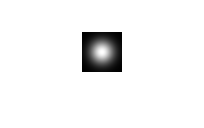
\includegraphics[width=0.44\linewidth]{gaussian2d.png}
            }
            \hfill
            \subfloat[]{%
              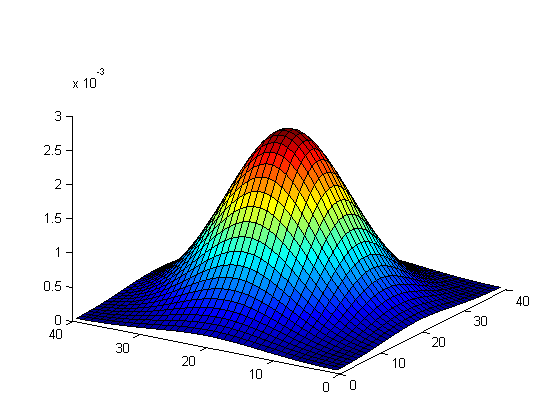
\includegraphics[width=0.44\linewidth]{gaussian3d.png}
            }
            \caption{PSF у випадку розмиття за Гаусом}
            \label{fig:gaussian-blur}
          \end{figure}
        \item Змазування (див.~Рис.~\ref{fig:gaussian-blur}).
          Цей вид розмиття спостерігається, коли в момент фотографування
          фотоапарат був швидко зміщений у просторі.
          Як видно з малюнку, кожен піксель трансформується у певну смугу, що
          відтворює характер руху.
          При цьому виді спотворення дуже важко встановити початкові пропорції
          об’єкту.
          \begin{figure}[ht!]
            \subfloat[]{%
              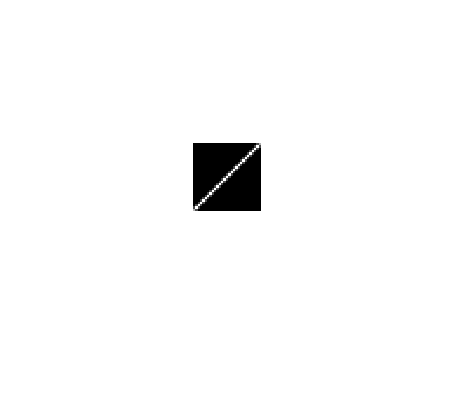
\includegraphics[width=0.44\linewidth]{motion2d.png}
            }
            \hfill
            \subfloat[]{%
              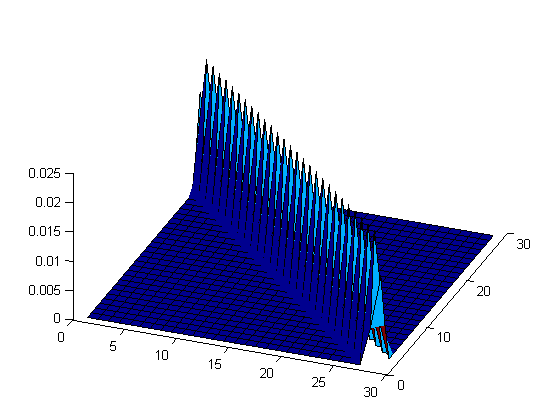
\includegraphics[width=0.44\linewidth]{motion3d.png}
            }
            \caption{PSF у випадку змазуванняу}
            \label{fig:motion-blur}
          \end{figure}
        \item Розмиття у формі диску (див.~Рис.~\ref{fig:disk-blur}).
          Цей вид розмиття дуже гарно описує ефект, відомий як Боке.
          Результат такого спотворення полягає в перетворенні кожного пікселю
          на коло певного радіусу з однаковою інтенсивністю.
          \begin{figure}[t]
            \subfloat[]{%
              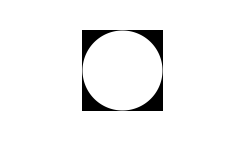
\includegraphics[width=0.44\linewidth]{disk2d.png}
            }
            \hfill
            \subfloat[]{%
              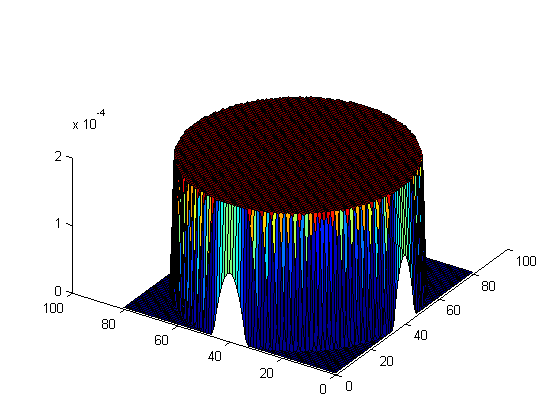
\includegraphics[width=0.44\linewidth]{disk3d.png}
            }
            \caption{PSF у випадку боке}
            \label{fig:disk-blur}
          \end{figure}
      \end{itemize}
    \subsection{Модель шуму}
      Цифровий шум --- дефект зображення, що вноситься фотосенсорами.
      Шум можна помітити на зображенні у вигляді певної маски з пікселей
      випадкового кольору та яскравості.
      На більшості сучасних камерах, у яких використовується масив цвітних
      фільтрів, шум має вигляд зерна, більш великого, ніж пікселі зображення.

      Кольоровий шум візуально забарвлює зображення, адже шум може мати різну
      інтенсивність для різних каналів зображення.
      Наприклад, шум на фотографії, що було знята при лампах накалювання, має
      більш жовто"=сині відтінки.\cite{honsales-woods}

      Шум помітно в однотонних областях, в особливості --- в темних областях.

      Зазвичай кажуть про співвідношення сигнал"=шум.
      На це співвідношення впливають шуми аналогової електроніки фотоапарату
      (посилювачі, АЦП), але основним джерелом цифрового шуму є фотосенсор.

      Причини шуму в цифрових сенсорах можуть бути самими різними:
      \begin{itemize}
        \item Дефекти (домішки та інші) потенціального бар’єру.
          Такі дефекти відображаються у вигляді чорних точок на світлому фоні.
        \item Темновий струм.
          На темному фоні відображається у вигляді світлих точок.
          Основна причина виникнення темнових струмів полягає в домішках у
          кремнієвій пластині.
        \item Через шум, що виникає внаслідок стохастичної природи взаємодії
          фотонів світла з атомами матеріалів фотодіодів сенсору.
        \item Через наявність дефектних пікселів, що виникають під час
          виробництва через недосконалість технології.
      \end{itemize}

      На величину шуму також впливає ряд факторів, а саме: значення ISO, тип
      матриці, розмір пікселя, температура, електромагнітні наведення тощо.
      У більшості випадків шум розподілений за законом Гауса(який задається
      двома параметрами --- математичним очікуванням і дисперсією):
      \begin{equation}
        f\left( x; \mu; \sigma \right) = \frac{1}{\sigma \sqrt{2 \pi}}
        e^{-\frac{\left( x - \mu \right)^2}{2 \sigma^2}}
        \label{eq:gaussian-blur}
      \end{equation}

      Цей шум характеризується рівномірною спектральною щільністю, нормально
      розподіленим значенням амплітуди та адитивним способом впливу на сигнал.

      Термін ,,адитивний'' означає, що даний шум підсумовується з
      корисним сигналом.

      Також важливим припущенням щодо шуму є те, що він не корелює з
      зображенням й не залежить від координат пікселю.
      \clearpage
  \section{Методи відновлення}
    Процеси, спрямовані на те, щоби усунути деградації з сигналів (не лише
    тих, що обумовлені згорткою) називають процесами відновлення.
    Одним з таких процесів є деконволюція.

    \subsection{Обернена згортка як метод відновлення}
      Деконволюція, або обернена згортка --- операція, що є оберненою до
      згортки двох сигналів.
      Можливість ,,пере"=фокусувати'' розмите зображення після того, як воно
      було зняте (використовуючи певні обчислення) може бути надзвичайно
      корисним, наприклад, коли неможливо зняти заново фотографію.

      Деконволюція має за собою мету обернути деградації сигналів, що були
      отримані через операцію згортки.
      Існують й інші види деградацій, але обернена згортка, зазвичай, не в
      змозі допомогти із ними.

      Оскільки цей процес намагається отримати сигнал до того, як він зазнав
      певної деградації, маючи лише цей деградований сигнал, деконволюція може
      бути класифікована як зворотна задача, а отже й математичні методи для
      зворотних задач тісно пов’язані з розумінням та розробкою алгоритмів
      деконволюції.

      \begin{figure}
        \subfloat[Початкове зображення]{%
          
\includegraphics[width=0.32\textwidth]{Aorig.png}
          \label{fig:deconvolution-example:orig}
        }
        \hfill
        \subfloat[Розмите зображення]{%
          
\includegraphics[width=0.32\textwidth]{AOrig.jpg}
          \label{fig:deconvolution-example:conv}
        }
        \hfill
        \subfloat[Відновлене зображення]{%
          
\includegraphics[width=0.32\textwidth]{ADecon.jpg}
          \label{fig:deconvolution-example:deconv}
        }
        \caption{Приклад деконволюції}
        \label{fig:deconvolution-example}
      \end{figure}

      Приклад роботи деконволюції зображення наведений на
      рис.~\ref{fig:deconvolution-example}.
      Як видно з цієї ілюстрації, процес оберненої згортки відновив багато
      деталей, що були ,,втрачені'' під час розмиття.
      Також треба звернути увагу на те, що відновлене зображення має певні
      вкраплення, які були відсутні на початковому зображенні.
      Ці вкраплення є прикладом артефактів (небажаним ,,побічним ефектом'')
      деконволюції.\cite{deconvolve-index}
      \paragraph{Взаємозамінність згортки та деконволюції}
        Операція згортки не завжди пов’язана з деградацією сигналу.
        Насправді, за допомогою ,,правильної'' PSF, згортка може прибрати розмиття
        зображення, а також проста згортка з так званим зворотним фільтром
        може фактично зробити деконволюцію попереднього перетворення.

        Таким чином, згортка та деконволюція при певних умовах можуть виконувати
        однакові дії.
      \clearpage
    \subsection{Види деконволюції}
      Деконволюцію можна класифікувати за інформацією, що відома про функцію
      розсіювання точки:
      \begin{itemize}
        \item Несліпа.
          У цьому випадку функція розподілу точки відома до початку
          застосування алгоритму.
          Найчастіше це можна отримати після моделювання всієї оптичної
          системи.
          Ці методи вирішують класичну обернену задачу, колу відомі всі
          доданки, окрім одного.
          Алгоритми цієї групи досить корисні, адже не вони використовуються у
          більш складної, сліпої деконволюції.
        \item Сліпа.
          У цьому випадку функція розсіювання точки не відома заздалегідь, а
          тому потрібно використовувати інші методи відновлення зображення.
          Ця задача є набагато складнішою за несліпу деконволюцію, адже
          необхідно знайти оригінал зображення лише за деградованим зображенням.
          Для того, щоб рішення цієї задачі було можливим необхідно вказати
          певні межі можливого розв’язку.
          Насправді, вказувати межі може бути необхідно й при вирішенні задачі
          несліпої деконволюції, адже часто існує багато різних розв’язків.
        \item Випадки, коли відома частина PSF.
          У цьому випадку задачу відновлення можна розділити на певні
          підзадачі, сліпі й несліпі, й вирішувати їх окремо.
      \end{itemize}
      \clearpage
  \section{Методи несліпої деконволюції}
    \subsection{Інверсна фільтрація}
      Одним з найочевидніших рішень є ділення всього
      рівняння~\eqref{eq:deffect-fourier} на $H\left( u, v \right)$, в
      результаті чого ми отримаємо наближення до початкового зображення
      $\hat{F}\left( u, v \right)$:

      \begin{equation}
        \hat{F}\left( u, v \right) = F\left( u, v \right) + \frac{N\left( u, v
        \right)}{H\left( u, v \right)}
        \label{eq:inverse-filter:idea}
      \end{equation}

      Це рівняння описує процес, що має назву інверсна фільтрація.
      Тобто, інверсна фільтрація полягає в
      \begin{itemize}
        \item Перетворенні Фур’є, що переводить систему до частотної області.
        \item Ділення образу перетворення Фур’є від вхідного зображення на
          образ Фур’є функції розподілу точки:
          \begin{equation}
            \hat{F}\left( u, v \right) = \frac{G\left( u, v \right)}{H\left(
            u, v \right)}
            \label{eq:inverse-filter}
          \end{equation}
        \item Зворотному перетворенні Фур’є від $\hat{F}\left( u, v \right)$.
      \end{itemize}
      Проте, на практиці він майже ніколи на приводить до гарного результату.
      Для того, щоб зрозуміти, чому так трапляється, достатньо подивитися на
      останній доданок з рівняння~\eqref{eq:inverse-filter} --- якщо функція $H\left(
      u, v \right)$ приймає значення, близькі до нульових, то цей доданок буде
      домінуючим.
      Саме так і трапляється на практиці.\cite{honsales-woods-eddins}
      \clearpage
    \subsection{Фільтр Вінера}
      Існують методи, що враховують існування шуму на зображенні.
      Один з самих відомих й старіших --- фільтр Вінера (Wiener).

      В математичній моделі алгоритму Вінера як зображення, так і шум
      розглядаються як випадкові (стохастичні) процеси.
      Основна ідея --- знайти таку оцінку $f^\prime$ неспотвореного
      (початкового) зображення $f$, таку, щоб середньоквадратичне відхилення
      цих величин було мінімальним.

      Вінер знайшов, що мінімум цього відхилення досягається на функції в
      частотній області:
      \begin{equation}
        \hat{F}\left( u, v \right) = \left( \frac{1}{H\left( u, v \right)}
        \frac{\left| H\left( u, v \right)\right|}{\left|H\left( u, v
          \right)\right|^2 + \frac{S_\eta\left( u, v \right)}{S_f\left( u, v
          \right)}} \right) G\left( u, v \right)
        \label{eq:wiener1}
      \end{equation}

      Функцією $S$ тут позначені енергетичні спектри шуму та початкового
      зображення.
      Оскільки ці величини майже ніколи не відомі, то доданок
      $\frac{S_\eta}{S_f}$ замінюють на деяку константу $K$, яку можна
      охарактеризувати як співвідношення сигналу до шуму.

      Всі дії в алгоритмі Вінера виконуються в частнотній області, а тому
      потрібно застосувати перетворення Фур’є до початкових даних, а потім
      застосувати обернене перетворення Фур’є до результату.
      \clearpage
    \subsection{Фільтрація за Тихоновим}
      Розглянемо наступний метод --- фільтрація за Тихоновим, або
      регуляризація за Тихоновим.
      Його ідея полягає в формулюванні завдання в матричному вигляді та
      подальшому рішенні отриманої задачі оптимізації.

      Це рішення записується у вигляді:
      \begin{equation}
        \hat{F}\left( u, v \right) = \left( \frac{H^\ast\left( u, v
        \right)}{\left|H\left( u, v \right)\right|^2 + y\left|P\left( u, v
        \right)\right|^2} \right) G\left( u, v \right)
        \label{eq:tihonov1}
      \end{equation}

      У рівнянні~\eqref{eq:tihonov1} $y$ --- параметр регуляризації, а
      $P\left( u, v \right)$ --- перетворення Фур’є оператору Лапласу (матриця
      $3\times3$).
    \subsection{Метод Люсі"=Річардсона}
      Ще одне досить цікаве рішення було незалежно знайдене Річардсоном у
      1972~році та Люсі у 1974~році.
      Його головною особливістю є те, що він не є лінійним, на відміну від
      попередніх.
      Через це він, потенціально, може дати кращий результат.
      Друга особливість --- цей метод є ітеративним, через це існують деякі
      складності, що пов’язані з критерієм зупинки ітерацій.

      Основна ідея полягає в використанні методу максимальної
      правдоподібності, для чого припускається, що спотворююча функція
      описується певним розподілом Пуасону.

      Також, на відміну від попередніх методів, перетворення Фур’є не
      використовується в цьому методі:
      \begin{equation}
        \hat{f}_{k+1}\left( x, y \right) = \hat{f}_k \left( x, y \right)\left(
        h\left( -x, -y \right) \ast \frac{g\left( x, y \right)}{h\left( x, y
          \right) \ast \hat{f}_k\left( x, y \right)} \right)
        \label{eq:lr1}
      \end{equation}

      Цей метод набув широкого застосування для обробки астрономічних
      фотознімків --- у цей сфері використання деконволюції, як методі
      відновлення зображення, є стандартом де-факто.
      Обчислювальна складність методу досить велика --- обробка середньої
      фотографії, в залежності від кількості ітерацій, може займати години й
      навіть дні.

      Алгоритм можна записати у трохи іншому, більш легкому для реалізації,
      вигляді.
      Точки розмитого зображення можуть бути представленими у формі суми:
      \[ d_i = \sum_j p_{ij} u_j, \]
      де $p_{ij}$ --- частина інтенсивності, що розсіялася з позиції $j$ в
      позицію $i$, а $u_j$~"--- $j$-та точка зображення, $d_i$ --- $i$-та точка
      отриманого розмитого зображення.\cite{richardson-hadley}

      Головна ідея полягає в тому, що необхідно підрахувати найбільш"=вірогідне
      значення $u_j$, якщо відомі $d_i$ та $p_{ij}$.

      \begin{equation}
        u_j^{(t+1)} = u_j^{(t)} \sum_i \frac{d_i}{c_i} p_{ij}
        \label{eq:rl-deconv}
      \end{equation}

      \[c_i = \sum_j p_{ij} u_j^{(t)}\]
      \clearpage
  \section{Методи сліпої деконволюції}
    Зараз набуває популярності сімейство методів, об’єднані під загальною
    назвою сліпа деконволюція (blind deconvolution).

    В попередніх методах вважалося, що функція спотворення PSF відома.
    Але в реальності найчастіше PSF відома лише приблизно за характером
    спотворення.
    Сліпа деконволюція як раз має за собою мету врахувати цей факт.

    Принцип у багатьох випадках досить простий:
    \begin{itemize}
      \item Знаходиться деяке наближення функції розподілу точки.
      \item Далі, за одним із методів несліпої деконволюції зображення
        відновлюється.
      \item Після цього за певними критеріями оцінюється ступінь якості
        відновленого зображення й уточнюється PSF для подальшої ітерації.
    \end{itemize}

    Основна складність цього методи полягає в критерії якості зображення й
    методах уточнення функції розподілу точки.
    \clearpage
  \section{Методи наближення функції розподілу точки}
    \subsection{Побудова PSF за фізичними параметрами об’єктивів}
      Основна ідея цього методу полягає в вивченні характеристик усіх оптичних
      елементів фотоапарату й подальшому моделюванні шляху світла через них.

      Моделювання PSF є дуже непростою й трудомісткою проблемою.

      Сучасні об’єктиви складаються з десятків різних оптичних лінз та оптичних
      елементів, частина з яких мають асферичну форму.
      Також, кожен сорт скла, з якого виготовляються лінзи, має свої унікальні
      характеристики заломлення променів із тією чи іншою довжиною хвилі.

      Отже, задача моделювання PSF в такій складній оптичній системі, з
      урахуванням впливу діафрагм, перевідбиттів тощо стає практично неможливою
      задачею.

      Рішення цієї задачі доступно лише, можливо, розробникам сучасних
      об’єктивів.
      \clearpage
    \subsection{Безпосереднє спостереження}
      Ідея цього методу полягає в безпосередньому спостереженні перетворення
      точки під час спотворення.

      Оскільки PSF показує, на що перетворюється кожна точка початкового
      зображення, можливо отримати шукану PSF отримавши зображення білої точки
      на чорному фоні після спотворення.

      Хоча цей метод здається простим, існує багато нюансів.
      Наприклад, PSF може бути різною для хвиль різної довжини.
      PSF може залежати від координат пікселю.

      Також потрібно пам’ятати, що знайдена таким чином PSF буде правдивою
      лише при тому ж самому спотворенні, що в багатьох випадках складно
      отримати.
      \clearpage
    \subsection{Обчислення або непряме спостереження}
      Цей метод напряму залежить від можливості отримати неспотворене
      зображення, а отже має дуже малу область застосування.

      З формули~\eqref{eq:deffect-fourier} можна отримати образ перетворення
      Фур’є від функції розподілу точки $H\left( u, v \right)$ як результат
      ділення образу Фур’є спотвореного зображення $G\left( u, v \right)$ на
      Фур’є перетворення від початкового зображення $F\left( u, v \right)$.

      Цей метод показує, що ми можемо розглядати початкове зображення $f\left(
      x, y \right)$ як функції спотворення для $h\left( x, y \right)$

      Для найкращого ефекту необхідно поставити фотоапарат на штатив й
      сфотографувати певний об’єкт, після чого зробити розмитий знімок того ж
      самого об’єкту з тієї ж самої позиції.
      \clearpage
    \subsection{Боке}
      Розглянемо трохи теорії розфокусування стосовно реальної оптики.

      Ідеальний об’єктив має PSF у вигляді кола, відповідно кожна точка
      перетворюється в коло деякого діаметру.
      До речі, саме через це з першого погляду здається, що дефокус просто
      розтушовує все зображення.
      Це ж пояснює і те, чому розмиття за Гаусом, здійснене у фоторедакторах
      зовсім не схоже на той малюнок фону (його ще називають боке), який
      ми бачимо у об’єктивів.
      Насправді це два різних типи розмиття --- за Гаусом кожна точка
      перетворюється на нечітка пляма (дзвін Гауса), а дефокус кожну точку
      перетворює в коло.
      Відповідно і різні результати.

      Але ідеальних об’єктивів не існує, і в реальності ми отримуємо те чи інше
      відхилення від ідеального кола.
      Саме це і формує неповторний малюнок боке кожного об’єктива.

      \begin{figure}[h]
        \subfloat[Нейтральне боке]{%
          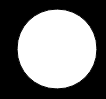
\includegraphics[width=0.32\textwidth]{neutral_boke.png}
          \label{fig:boke:neutral}
        }
        \hfill
        \subfloat[М’яке боке]{%
          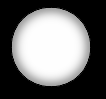
\includegraphics[width=0.32\textwidth]{soft_boke.png}
          \label{fig:boke:soft}
        }
        \hfill
        \subfloat[Жорстке боке]{%
          
\includegraphics[width=0.32\textwidth]{hard_boke.png}
          \label{fig:boke:hard}
        }
        \caption{Види боке}
        \label{fig:boke}
      \end{figure}

      Боке можна умовно розділити на три типи:
      \begin{itemize}
        \item Нейтральне. Це максимальне наближення до кола.
        \item М’яке. Коли краю мають меншу яскравість, ніж центр
        \item Жорстке. Коли краю мають велику яскравість, ніж центр.
      \end{itemize}
      Крім того, тип боке залежить від того, чи передній це фокус, чи
      задній.
      Тобто, чи фотоапарат сфокусований перед об’єктивом чи за ним.
      Тільки нейтральне боке не залежить від фокусу.

      \clearpage
\chapter{МАТЕМАТИЧНЕ МОДЕЛЮВАННЯ}
  У процесі спотворення з кожного пікселя вихідного зображення виходить деяке
  пляма у разі розфокусуванні і відрізок для випадку звичайного змазуванняу.
  Все це один на одного накладається і в результаті ми отримуємо спотворене
  зображення ---- це називається згорткою, або конволюцієй, зображення.
  Те, за яким законом розмазуванняується один піксель і називається функцією
  спотворення.
  Інші синоніми --- PSF (Point spread function, тобто функція розподілу
  точки), ядро оператора спотворення, kernel та інші.

  Щоб відновити вихідне зображення нам необхідно якимось чином обернути процес
  згортки, при цьому не забуваючи про шум.
  Але це не така проста задача --- якщо діяти, що називається, ,,напряму'', то
  вийде величезна система рівнянь, яку вирішити за прийнятний час неможливо.
  \section{Додатковий математичний апарат}
    Для подальшої роботи потрібно додатково розібрати математичний апарат, що
    буде викладений нище.
    \subsection{Згортка у двовимірному просторі}
      Для зображення, розміром $M \times N$ та PSF розмірністю $m \times n$,
      згортка приймає вид, наведений у~\eqref{eq:convolution-2d}.\cite{knuth}
      \begin{equation}
        g\left( x, y \right) = h\left( x, y \right) \ast f\left( x, y \right)
        = \sum_{i=-a}^a \sum_{j = -b}^b h\left( i, j \right) f\left( x + i, y
        + j \right).
        \label{eq:convolution-2d}
      \end{equation}

      У рівнянні~\eqref{eq:convolution-2d} константи $a$ і $b$ визначаються з
      наступних формул:
      \begin{equation*}
        a = \frac{m - 1}{2}, b = \frac{n - 1}{2}
      \end{equation*}
    \subsection{Перетворення Фур’є}
      Перетворення Фур’є --- це інтегральне перетворення однієї комплекснозначної
      функції дійсної змінної на іншу.
      Тісно пов’язане з перетворенням Лапласа та аналогічне розкладу у ряд
      Фур’є для неперіодичних функцій.
      Це перетворення розкладає дану функцію на осциляторні функції.
      Перетворення Фур’є визначається за формулою~\eqref{eq:fourier-def}.
      Зворотна операція, обернене перетворення Фур’є, визначається
      формулою~\eqref{eq:invfourier-def}.
      \begin{equation}
        F\left( \omega \right) = \int_{-\infty}^\infty f\left( t \right) e^{-i
        \omega t }\,dt
        \label{eq:fourier-def}
      \end{equation}
      \begin{equation}
        f\left( t \right) = \frac{1}{2 \pi} \int_{-\infty}^\infty F\left(
        \omega \right) e^{i \omega t}\, d\omega
        \label{eq:invfourier-def}
      \end{equation}

      У дискретному випадку перетворення Фур’є приймає наступний вигляд:
      \begin{equation}
        X_k = \sum_{n = 0}^{N - 1} x_n e^{-\frac{2 \pi i}{N} k n} \quad k =
        0,\cdots, N - 1
        \label{eq:fourier-def-discrete}
      \end{equation}
      \begin{equation}
        x_n = \frac{1}{N} \sum_{k = 0}^{N - 1} X_k e^{\frac{2 \pi i}{N} k n}
        \quad n = 0,\cdots, N - 1
        \label{eq:invfourier-def-discrete}
      \end{equation}

      Одна з властивостей перетворення Фур’є --- перетворення Фур’є від
      згортки.
      Ящко $f\left( x \right)$, $g\left( x \right)$ та $h\left( x \right)$ ---
      інтегровані функції, а $F\left( \omega \right)$, $G\left( \omega
      \right)$
      та $H\left( \omega \right)$ --- їх відповідні перетворення Фур’є, то має
      місце наступне:
      \begin{quote}
        Якщо $h\left( x \right) = \left( f \ast g \right)\left( x \right)$,
        тоді $H\left( \omega \right) = F\left( \omega \right) G\left( \omega
        \right)$
      \end{quote}
      \paragraph{Наслідок з теореми про згортку}
        З рівняння~\eqref{eq:convolution-2d} видно, що для знаходження $f$ з $g$
        потрібно розв’язати велику систему рівнянь.
        Але, якщо скористатися теоремою про згортку та перетворення Фур’є,
        можна перейти від нетривіальної операції згортки в просторі до
        звичайного по елементному множенню у частнотній області.
        А саме, процес спотворення можна переписати наступним чином:
        \begin{equation}
          G\left( u, v \right) = H\left( u, v \right) F\left( u, v \right) +
          N\left( u, v \right)
          \label{eq:deffect-fourier}
        \end{equation}
      \clearpage
  \section{Практичний аналіз алгоритмів деконволюції}
    \subsection{Інверсна фільтрація}
      Інверсна фільтрація є дуже простим методом, але вона не передбачає
      наявності шуму у зображенні.

      Візьмемо початкове зображення, перетворимо його у напівтонове й
      отримаємо його спектр.
      \begin{figure}[ht]
        \subfloat[Початкове зображення]{%
          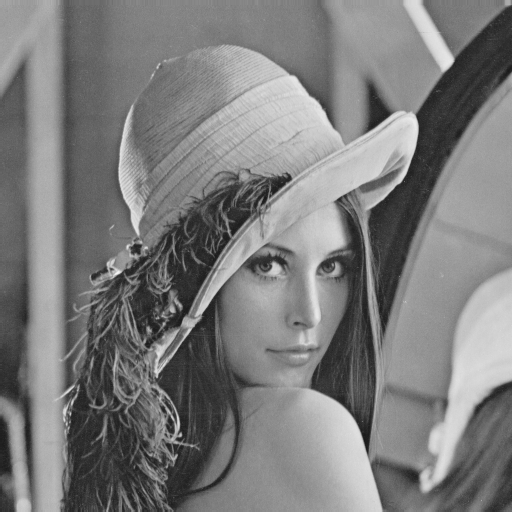
\includegraphics[width=0.32\textwidth]{Lenna-gray.png}
          \label{fig:Lenna:gray}
        }
        \hfill
        \subfloat[Амлітудний спектр]{%
          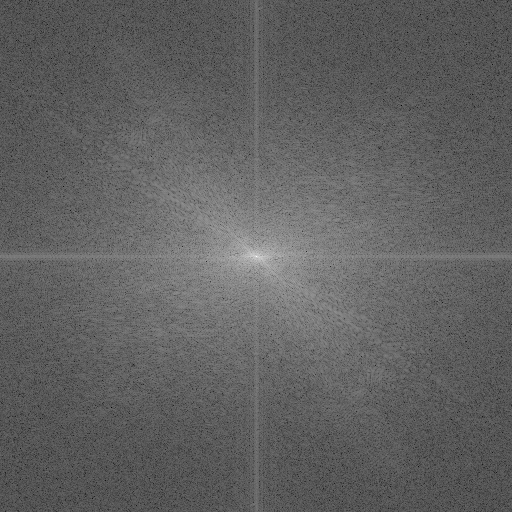
\includegraphics[width=0.32\textwidth]{Lenna-ampl.png}
          \label{fig:Lenna:ampl}
        }
        \hfill
        \subfloat[Фазовий спектр]{%
          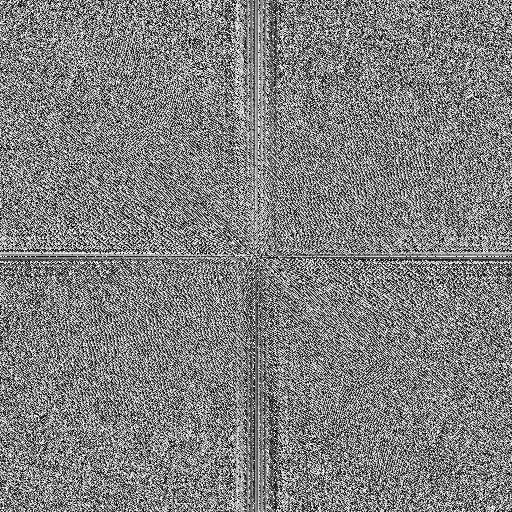
\includegraphics[width=0.32\textwidth]{Lenna-phase.png}
          \label{fig:Lenna:phase}
        }
      \end{figure}

      Як видно з амплітудного спектру, зображеному на
      Рис.~\ref{fig:Lenna:ampl}, його значення змінюється дуже швидко ---
      на декілька порядків.
      В центрі --- максимальне значення (порядку $10^6$) та швидко зменшується
      до нульових по краях.
      Саме через це інверсна фільтрація буде працювати лише при нульових або
      близько нульових значеннях шуму.

      Візьмемо зображення~\ref{fig:Lenna:img}.
      Після розмиття, отримуємо результат, зображений на
      малюнку~\ref{fig:Lenna:blurred}.
      Застосувавши інверсну фільтрацію, отримаємо відновлене
      зображення~\ref{fig:Lenna:invfilter}.

      \begin{figure}[ht]
        \subfloat[Початкове зображення]{%
          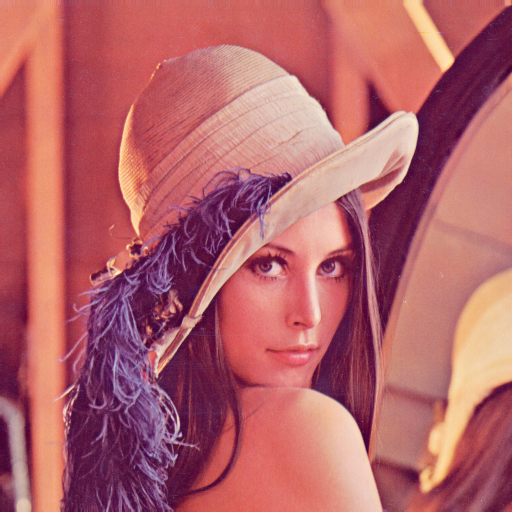
\includegraphics[width=0.32\textwidth]{Lenna.png}
          \label{fig:Lenna:img}
        }
        \hfill
        \subfloat[Розмите зображення]{%
          
\includegraphics[width=0.32\textwidth]{Lenna-blurred.png}
          \label{fig:Lenna:blurred}
        }
        \hfill
        \subfloat[Відновлене зображення]{%
          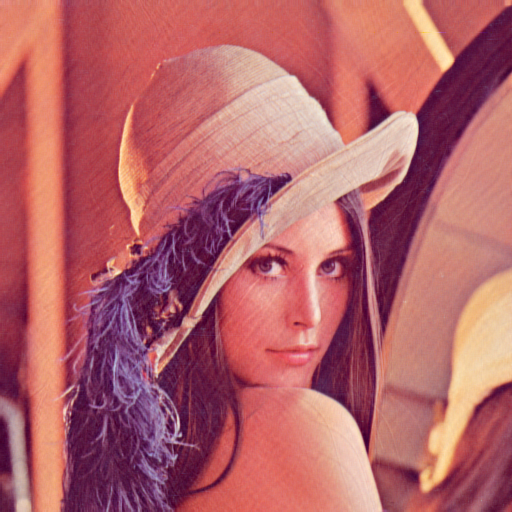
\includegraphics[width=0.32\textwidth]{Lenna-b0deconv.png}
          \label{fig:Lenna:invfilter}
        }
      \end{figure}

      Додамо до розмитого зображення~\ref{fig:Lenna:blurred} досить малий
      рівень шуму (див. рис.~\ref{fig:Lenna:blurred:10-9}).
      Після відновлення отриманий результат (див.
      рис.~\ref{fig:Lenna:invfilter:10-9}) майже не відрізняється від
      зображення, що ми отримали, відновивши зображення без шуму.

      \begin{figure}[htb]
        \hfill
        \subfloat[Зображення з шумом $10^{-9}$]{%
          
\includegraphics[width=0.32\textwidth]{Lenna-b1e-9.png}
          \label{fig:Lenna:blurred:10-9}
        }
        \hfill
        \subfloat[Відновлене зображення з шумом $10^{-9}$]{%
          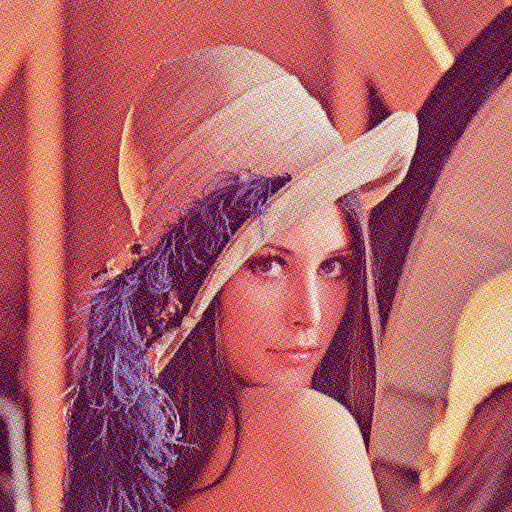
\includegraphics[width=0.32\textwidth]{Lenna-b1e-9deconv.png}
          \label{fig:Lenna:invfilter:10-9}
        }
        \hfill
      \end{figure}

      Але якщо додати до зображення трохи більший рівень шуму ($5\cdot10^{-9}$
      на малюнках~\ref{fig:Lenna:5-9} та $10^{-8}$ на
      малюнках~\ref{fig:Lenna:10-8}) отримаємо результати, що дуже сильно
      відрізняється від оригіналу через високий рівень шуму.
      \begin{figure}[htb]
        \subfloat[Зображення з шумом]{%
          
\includegraphics[width=0.32\textwidth]{Lenna-b5e-9.png}
          \label{fig:Lenna:blurred:5-9}
        }
        \hfill
        \subfloat[Відновлене зображення]{%
          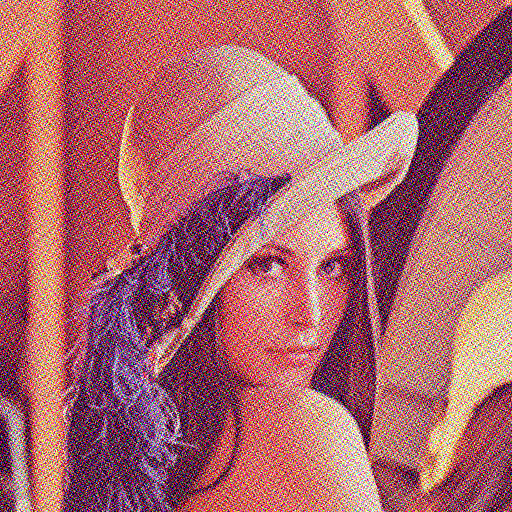
\includegraphics[width=0.32\textwidth]{Lenna-b5e-9deconv.png}
          \label{fig:Lenna:invfilter:5-9}
        }
        \hfill
        \caption{Вплив шуму $5\cdot10^{-9}$}
        \label{fig:Lenna:5-9}
      \end{figure}

      \begin{figure}[htb]
        \subfloat[Зображення з шумом]{%
          
\includegraphics[width=0.32\textwidth]{Lenna-b1e-8.png}
          \label{fig:Lenna:blurred:10-8}
        }
        \hfill
        \subfloat[Відновлене зображення]{%
          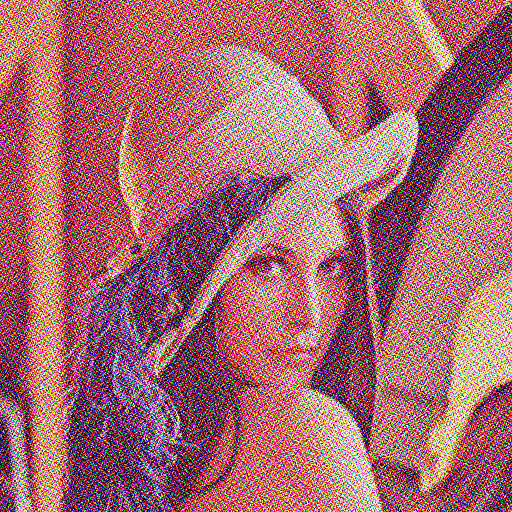
\includegraphics[width=0.32\textwidth]{Lenna-b1e-8deconv.png}
          \label{fig:Lenna:invfilter:10-8}
        }
        \hfill
        \caption{Вплив шуму $10^{-8}$}
        \label{fig:Lenna:10-8}
      \end{figure}
      Гарно видно, що додавання навіть дуже незначного шуму призводить до
      значних помилок, що сильно обмежує корисність методу.
      \clearpage
    \subsection{Регуляризація за Тихоновим}
      Одним із методів деконволюції, що враховують наявність шуму є
      Тихонівська регулярізація.

      Дослідимо, як цей метод відновлює різни види розмиття.
      \begin{figure}[ht]
        \subfloat[Розмите зображення]{%
          
\includegraphics[width=0.44\textwidth]{Lenna-disk.png}
          \label{Lenna:regul:disk:1}
        }
        \hfill
        \subfloat[Відновлене зображення]{%
          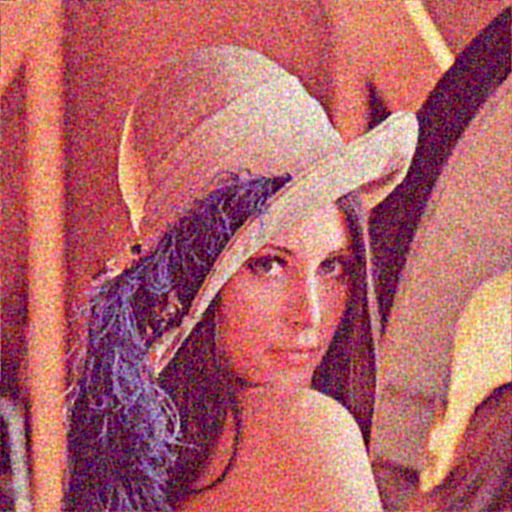
\includegraphics[width=0.44\textwidth]{Lenna-disk-regul.png}
          \label{Lenna:regul:disk:2}
        }
        \caption{Розмиття диском}
        \label{fig:regul:disk}
      \end{figure}

      \begin{figure}[ht]
        \subfloat[Розмите зображення]{%
          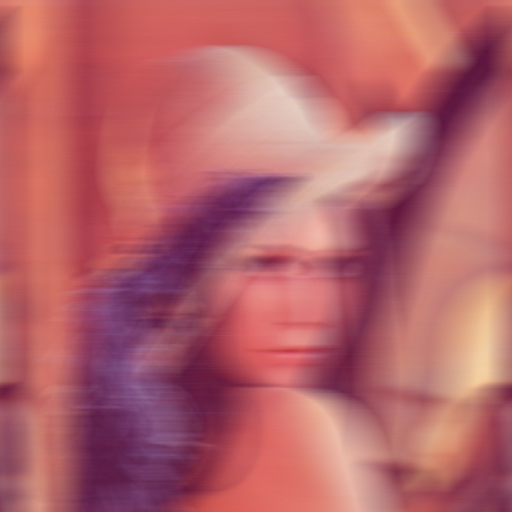
\includegraphics[width=0.44\textwidth]{Lenna-mot.png}
          \label{Lenna:regul:motion:1}
        }
        \hfill
        \subfloat[Відновлене зображення]{%
          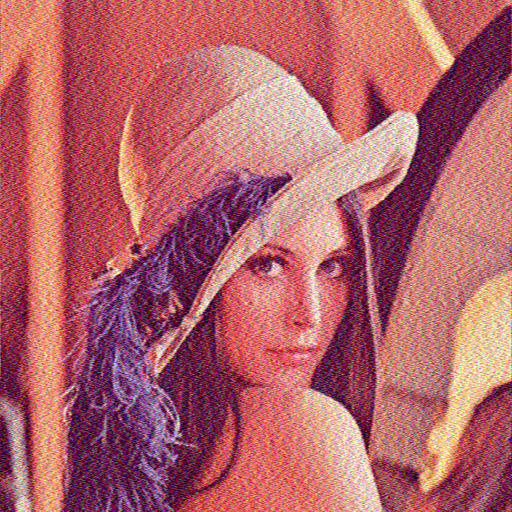
\includegraphics[width=0.44\textwidth]{Lenna-mot-regul.png}
          \label{Lenna:regul:motion:2}
        }
        \caption{Змазування}
        \label{fig:regul:motion}
      \end{figure}

      Як видно з рис.~\ref{fig:regul:disk}, цей метод відновлює загальну
      картину, але результат містить досить багато шумів.
      Окрім високого рівню відношення сигналу до шуму, на результаті не
      помітні інші артефакти.

      На рис.~\ref{fig:regul:motion} зображення, що було розмите рухом, метод
      Тихонова відновив досить цілісну картину, співвідношення сигналу до шуму
      менше, ніж у попередньому прикладі.

      Цей метод має невелику стійкість до шуму.
    \subsection{Фільтр Вінера}
      Фільтр Вінера є одним з найпоширеніших не ітераційних методів
      деконволюції.

      Дослідимо, як відновлюються зображення за допомогою цього методу.

      \begin{figure}[ht]
        \subfloat[Розмите зображення]{%
          
\includegraphics[width=0.44\textwidth]{Lenna-disk.png}
          \label{Lenna:wiener:disk:1}
        }
        \hfill
        \subfloat[Відновлене зображення]{%
          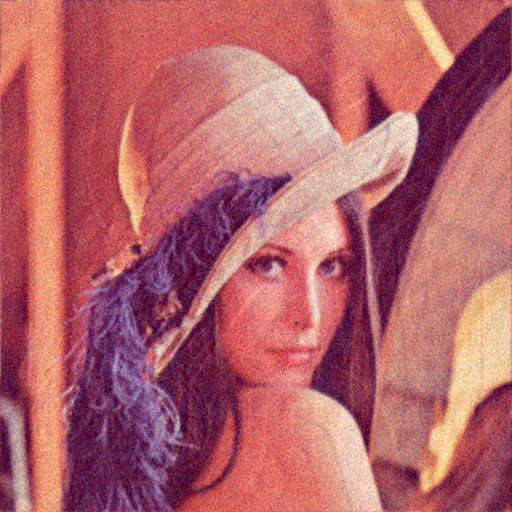
\includegraphics[width=0.44\textwidth]{Lenna-disk-wiener.png}
          \label{Lenna:wiener:disk:2}
        }
        \caption{Розмиття диском}
        \label{fig:wiener:disk}
      \end{figure}

      \begin{figure}[ht]
        \subfloat[Розмите зображення]{%
          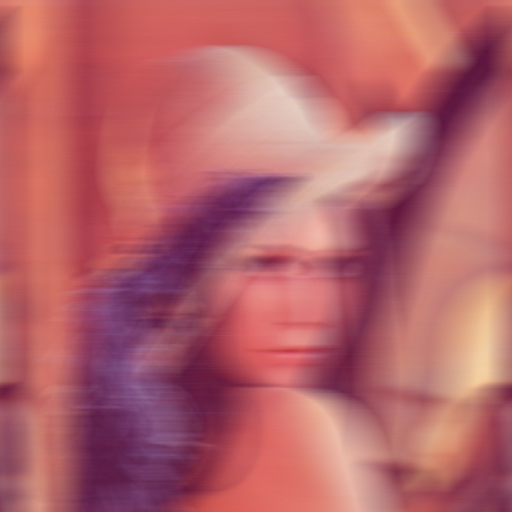
\includegraphics[width=0.44\textwidth]{Lenna-mot.png}
          \label{Lenna:wiener:motion:1}
        }
        \hfill
        \subfloat[Відновлене зображення]{%
          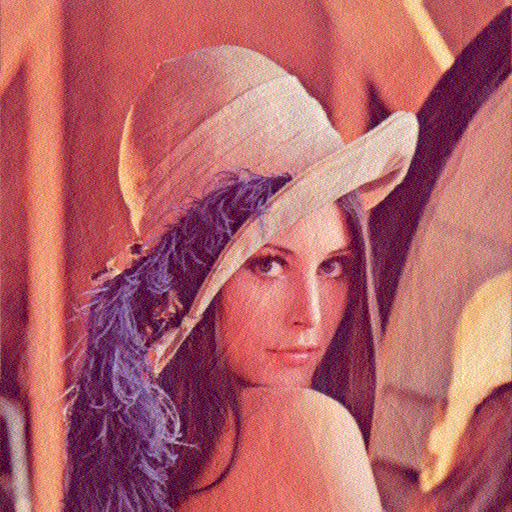
\includegraphics[width=0.44\textwidth]{Lenna-mot-wiener.png}
          \label{Lenna:wiener:motion:2}
        }
        \caption{Змазування}
        \label{fig:wiener:motion}
      \end{figure}

      Як видно з рис.~\ref{fig:wiener:disk}, метод відновлює зображення майже
      без шуму.
      Присутні лише деякі артефакти, такі, як подвійні границі.
      Але зображення дуже чітке й збережено всі деталі.

      На рис.~\ref{fig:wiener:motion} зображено відновлення зображення,
      розмитого змазуванням.
      Результат майже той самий, проте на цьому зображенні дуже мало
      артефактів.

      Як видно з цього прикладу, метод Вінера дуже гарно відновлює зображення
      (навіть з шумом), в особливості ті зображення, до були спотворені
      операцією зсуву.
      \clearpage
    \subsection{Алгоритм Люсі"=Річардсона}
      Цей алгоритм є єдиним алгоритмів, що застосовуються для рішення задачі
      деконволюції, що працює ітеративно.
      Також, однією з переваг цього методу є той факт, що він не вимагає
      перетворення Фур’є.
      Тобто, не потрібно робити перетворення Фур’є до початку алгоритму й
      обернене перетворення Фур’є після.

      Дослідимо, як відновлюються зображення за допомогою цього методу.

      \begin{figure}[ht]
        \subfloat[Розмите зображення]{%
          
\includegraphics[width=0.44\textwidth]{Lenna-disk.png}
          \label{Lenna:lucy:disk:1}
        }
        \hfill
        \subfloat[Відновлене зображення]{%
          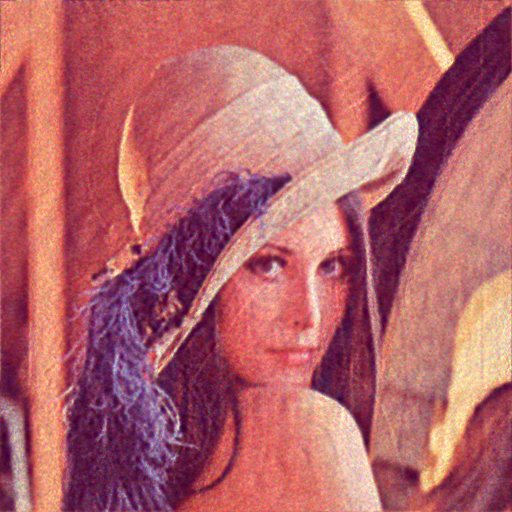
\includegraphics[width=0.44\textwidth]{Lenna-disk-lucy.png}
          \label{Lenna:lucy:disk:2}
        }
        \caption{Розмиття диском}
        \label{fig:lucy:disk}
      \end{figure}

      \begin{figure}[ht]
        \subfloat[Розмите зображення]{%
          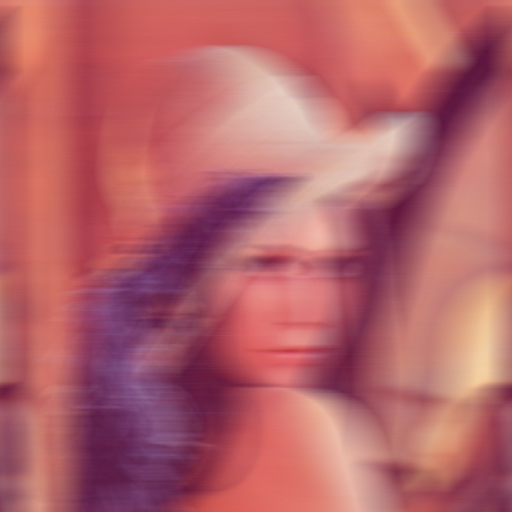
\includegraphics[width=0.44\textwidth]{Lenna-mot.png}
          \label{Lenna:lucy:motion:1}
        }
        \hfill
        \subfloat[Відновлене зображення]{%
          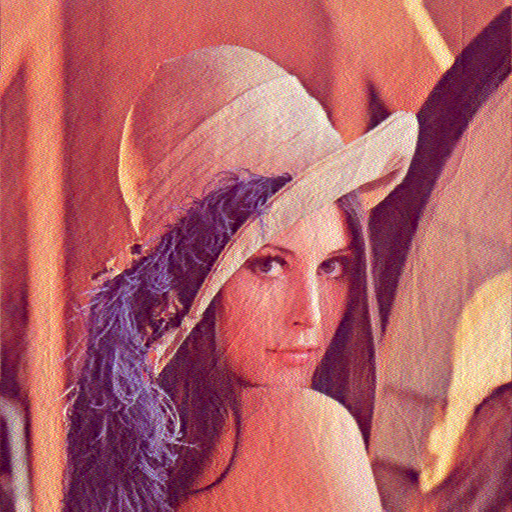
\includegraphics[width=0.44\textwidth]{Lenna-mot-lucy.png}
          \label{Lenna:lucy:motion:2}
        }
        \caption{Змазування}
        \label{fig:lucy:motion}
      \end{figure}

      Як видно з рис.~\ref{fig:lucy:disk}, метод відновлює зображення майже
      без шуму.
      Присутні лише деякі артефакти, такі, як подвійні границі.
      Але зображення дуже чітке й збережено всі деталі.
      В цілому, з таким розмиттям цей метод впорався трохи гірше за фільтр
      Вінера.

      На рис.~\ref{fig:lucy:motion} зображено відновлення зображення,
      розмитого змазуванням.
      Результат майже той самий, проте на цьому зображенні дуже мало
      артефактів.

      Як видно з цього прикладу, цей метод дозволяє отримати майже ті ж самі
      результати, що й фільтр Вінера, але потребує набагато більше часу.
      \clearpage
  \section{Підбор функції розподілу точки}
    Оцінка значення функції розподілу точки є досить досить цікавою проблемою.

    Можна оцінити загальний вид простої функції розподілу точки тільки за
    видом зображення, після чого необхідно підібрати параметри так, щоб
    відновити зображення як можна краще.

    \begin{figure}[ht]
      \centering
      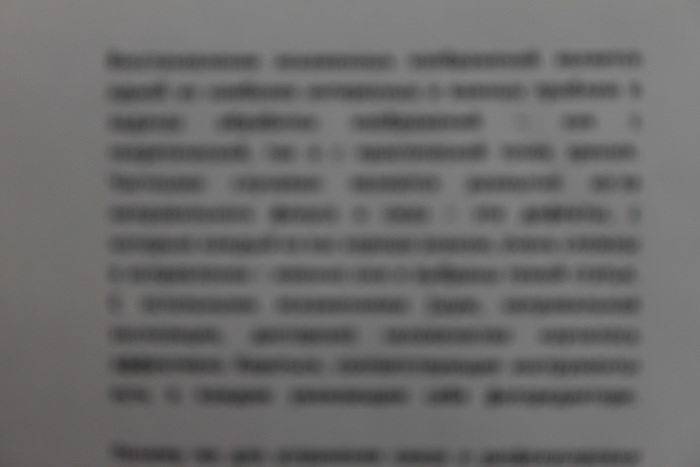
\includegraphics[width=0.8\linewidth]{text-blurred.jpg}
      \caption{Розфокусоване зображення}
      \label{fig:text:blurred}
    \end{figure}

    Наприклад, на рис.~\ref{fig:text:blurred} зображена розмита фотографія
    деякого тексту.
    Оскільки ми знаємо, що там зображений текст, ми можемо отримати після
    аналізу, що це зображення отримане через розфокусовання.
    Отже, для цієї фотографії ми визначили тип функції спотворення: диск
    (боке).
    Після цього слід підібрати єдиний параметр цієї функції --- радіус диску,
    у який розпливається кожен піксель зображення.
    Таким чином мною був отриманий досить непоганий результат при радіусі $70$
    пікселів (рис.~\ref{fig:text:unblurred}).

    \begin{figure}[ht]
      \centering
      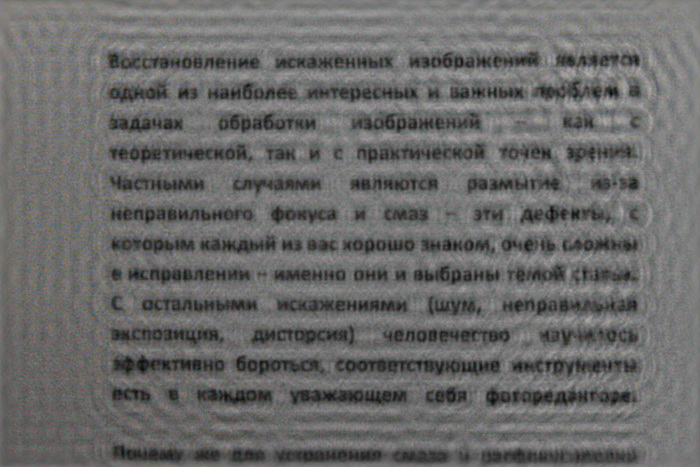
\includegraphics[width=0.8\linewidth]{text-unblurred.jpg}
      \caption{Відновлене зображення}
      \label{fig:text:unblurred}
    \end{figure}

    Розглянемо інше зображення, що було спотворене по іншому.

    \begin{figure}[hb]
      \centering
      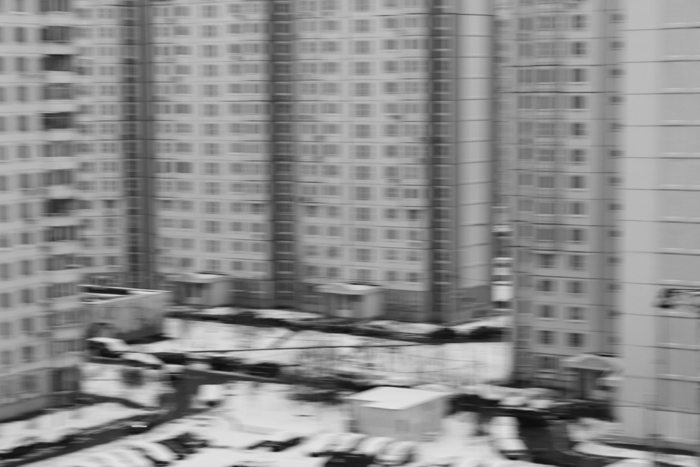
\includegraphics[width=0.80\linewidth]{house-mot.png}
      \caption{Змазане зображення}
      \label{fig:house:blurred}
    \end{figure}

    На рис.~\ref{fig:house:blurred} зображення спотворене через змазування.
    Оскільки ми знаємо приблизну геометричну форму, що мають дома, можна
    помітити, що один із параметрів розмиття змазування --- кут нахилу,
    дорівнює нулеві.
    Інший параметр, довжина змазу, треба підібрати емпірично.
    Наприклад, довжина змазу $14$ пікселей дозволяє відновити досить багато
    деталей зображення (рис.~\ref{fig:house:unblurred}).

    \begin{figure}[ht]
      \centering
      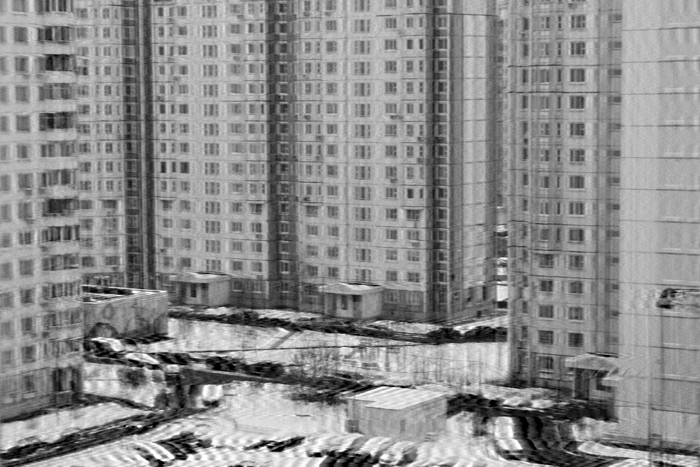
\includegraphics[width=0.8\linewidth]{house-unmot.png}
      \caption{Відновлене зображення}
      \label{fig:house:unblurred}
    \end{figure}
    \clearpage
  \section{Покращення результатів процесу відновлення}
    Описані методи можна й потрібно використовувати для побудови PSF при
    відновленні спотворених зображень.
    Оскільки від того, як добре ця функція наближена до реальної, залежить
    якість відновленого зображення.

    Якщо передбачувана та реальні PSF розбігаються, то будуть спостерігатися
    численні артефакти у вигляді ,,дзвону'', ореолів і зниження чіткості.
    У більшості випадків передбачається форма PSF у вигляді кола, проте для
    досягнення максимального ступеня відновлення рекомендується
    експериментувати з формою цієї функції, спробувавши кілька варіантів від
    поширених об’єктивів.

    Якщо безпосередньо застосувати фільтр Вінера, то на краях зображення буде
    своєрідний ,,дзвін''.
    Його причина полягає в наступному --- коли робиться деконволюція для тих
    точок, які розташовані на краях, то при складанні не вистачає даних з
    пікселів, які перебувають за краями зображення і вони приймаються або
    рівним нулю, або беруться з протилежного боку (залежить від реалізації
    фільтра Вінера і перетворення Фур’є). Виглядає це так:
    \begin{figure}[h]
      \centering
      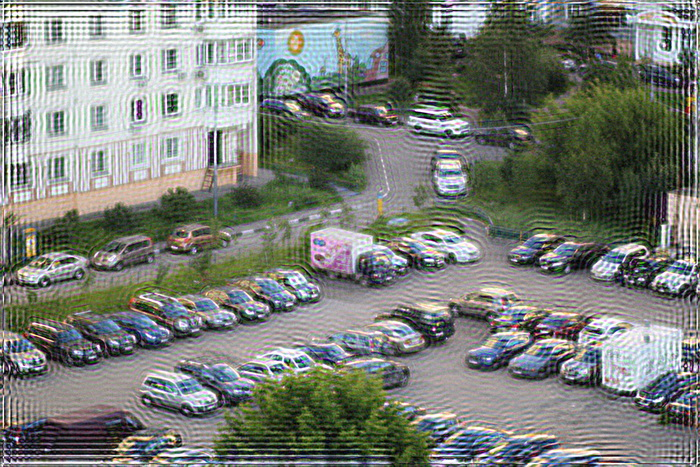
\includegraphics[width=\linewidth]{edge-artifact.jpg}
      \caption{Артефакт ,,дзвону''}
      \label{fig:edge-artifact}
    \end{figure}

    Одне з рішень полягає в попередній обробці країв зображення.
    Вони розмиваються за допомогою тієї ж самої функції розподілу точки.
    На практиці це реалізується наступним чином --- береться вхідне,
    спотворене, зображення $F\left( x, y \right)$, розмивається за допомогою
    PSF, тим самим отримуємо $F^\prime\left( x, y \right)$.
    Після цього отримуємо остаточне вхідне зображення як суму $F\left( x, y
    \right)$ та $F^\prime\left( x, y \right)$ з використанням вагової функції,
    яка по краях зображення приймає значення $1$, а всередині зображення,
    на відстані більше чи рівної радіусу PSF від країв зображення, приймає
    значення $0$.
    Результат отримуємо наступний (вже без ,,дзвону'' по краях):
    \begin{figure}[h]
      \centering
      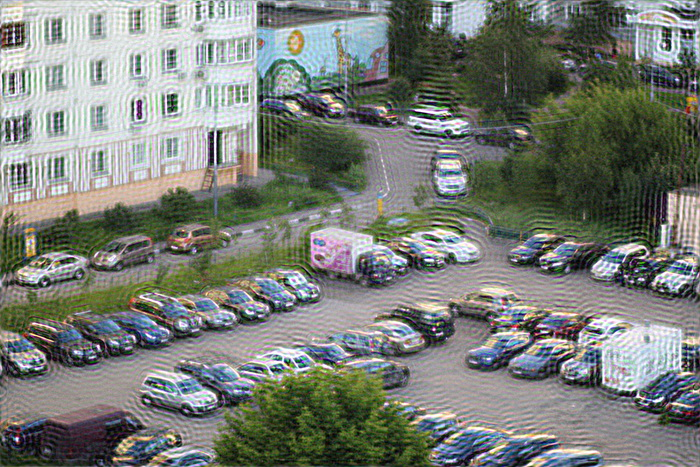
\includegraphics[width=\linewidth]{edge-fixed.jpg}
      \caption{Зображення без артефакту ,,дзвону''}
      \label{fig:edge-fixed}
    \end{figure}

\chapter{ПРОГРАМНА РЕАЛІЗАЦІЯ}
  Було розроблено пакет прикладних програм, що демонструють відновлення
  змазаних і розфокусованих зображень.

  У програмі було використано метод фільтру Вінера як метод відновлення
  зображення, адже цей алгоритм дозволяє досить точно відновити зображення
  навіть за наявності шуму.

  Були використані наступні технологічні рішення:
  \begin{itemize}
    \item мова програмування C++;
    \item набір бібліотек Qt4;
    \item бібліотека FFTW, як найшвидша реалізація перетворення Фур’є, що
      розповсюджується під ліцензією GPLv3.\cite{numerical}
  \end{itemize}

  \begin{figure}[h]
    \centering
    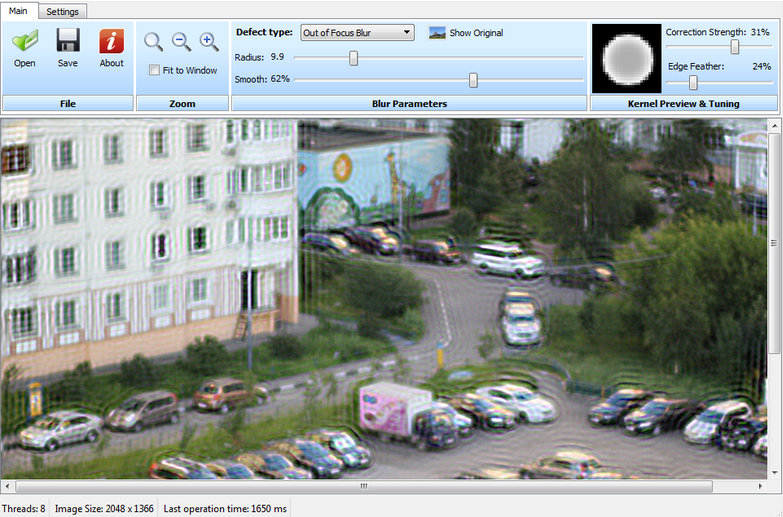
\includegraphics[width=\linewidth]{gui.png}
    \caption{Знімок екранної форми}
    \label{fig:gui}
  \end{figure}

  Основні можливості розробленого програмного засобу:
  \begin{itemize}
    \item Швидкодія.
      Обробка зображення розміром $2048\times1500$ пікселів займає близько
      $300$~мс в режимі Preview (коли можливо корегувати PSF) й $1500$~мс у
      фінальному режимі.
    \item Можливість вибору параметрів у Realtime режимі.
      Немає необхідності натискати кнопку Preview, усе робиться автоматично.
    \item Уся обробка проводиться над зображенням у повному розмірі.
    \item Можливість корегування PSF.
  \end{itemize}

  Програмний засіб дозволяє:
  \begin{itemize}
    \item Відкривати та зберігати зображення у форматах PNG, JPEG, BMP та
      інших.
    \item Масштабувати зображення: збільшувати, зменшувати та заповнювати всю
      екрану форму.
    \item Обирати бажаний вид функції спотворення: втрата фокусу, змазування.
    \item Корегувати параметри функції спотворення: радіус диска розмиття, кут
      нахилу та довжина змазу.
    \item Переглянути вид функції розподілу точки та дещо вдосконалити його,
      вказавши жорсткість країв.
    \item Проводити швидке відновлення під час підбору параметрів та більш
      детальне під час фінального проходу.
    \item Користуватися програмою під час обчислень.
  \end{itemize}

  Оскільки програмний засіб спрямований на користувача, який може дуже довго
  вибирати необхідні параметри функції розподілу точки, передбачені два режими
  відновлення: швидкий, у якому не використовуються ніякі додаткові методи
  покращення якості, та фінальний, який працює у 5--10 разів довше, але
  приводить до кращого результату.

  Також, щоб користувач міг комфортно працювати, усі перетворення швидкого
  методу відновлення відбуваються автоматично, після кожної зміни функції
  розподілу точки.
  Проте, всі обчислення проходять в окремому потоці, що дозволяє
  користувачеві поміняти якийсь параметр і тим самим запустити заново процес
  обчислень.

  Завдяки використанню тільки кросплатформних рішень, ця програма може
  використовуватись на багатьох видах операційних систем: Mac OS X, GNU/Linux,
  Windows.
  Також використання бібліотеки Qt дозволяє використовувати безліч форматів
  зображень у програмі.

  Алгоритм роботи програмного засобу зображений на рис.~\ref{fig:flowchart}.
  \begin{figure}[ht]
    \centering
    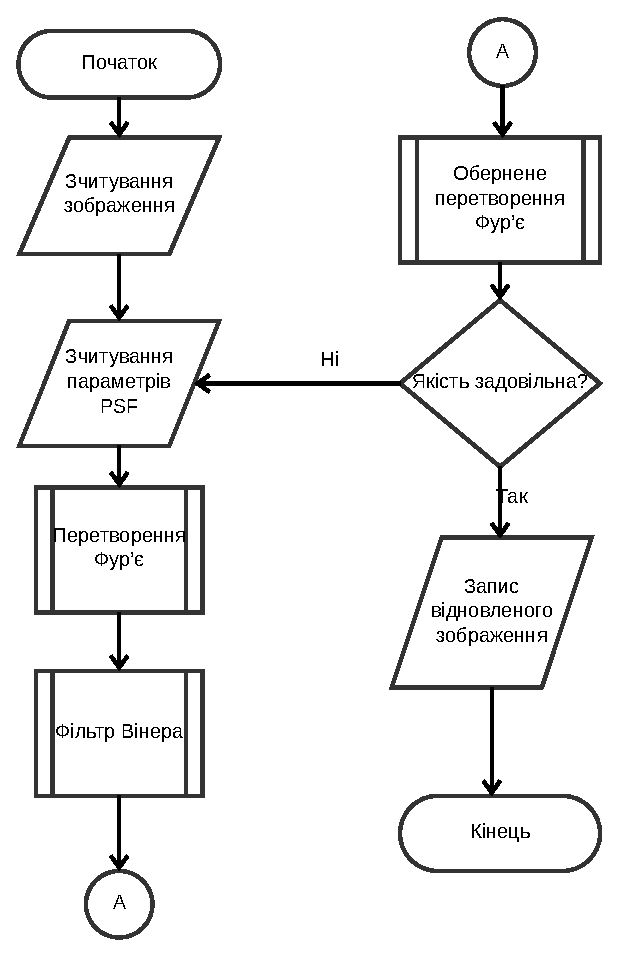
\includegraphics{flowchart.eps}
    \caption{Блок-схема алгоритму}
    \label{fig:flowchart}
  \end{figure}

\chapter{ОХОРОНА ПРАЦІ}
  За сучасних умов, комп’ютери набули широкого поширення.
  Вони застосовується на кожному підприємстві для організації діяльності
  праці.
  Комп’ютери є невід’ємним і, найчастіше, одним із головних інструментів при
  виконанні поставлених завдань.

  Даних розділ дипломної роботи носить рекомендаційний характер та має
  відношення до робіт одного типу, а отже подальші рекомендації будуть
  пов’язані зі специфікою роботи з персональними комп’ютерами.

  Основним нормативним документом щодо забезпечення охорони праці користувачів
  персонального комп’ютера є НПАОП~0.00-1.28-10\cite{npaop128} та
  ДНАОП~0.00-1.31-99\cite{dnaop131}.
  \section{Характеристика робочого місця}
    Робоче приміщення знаходиться на четвертому поверсі в цегляному будинку.
    Найближчі будівлі знаходяться на значній відстані та не впливають на
    рівень проникнення світла.
    План приміщення зображений на рис.~\ref{fig:plan}.
    \begin{figure}[ht]
      \centering
      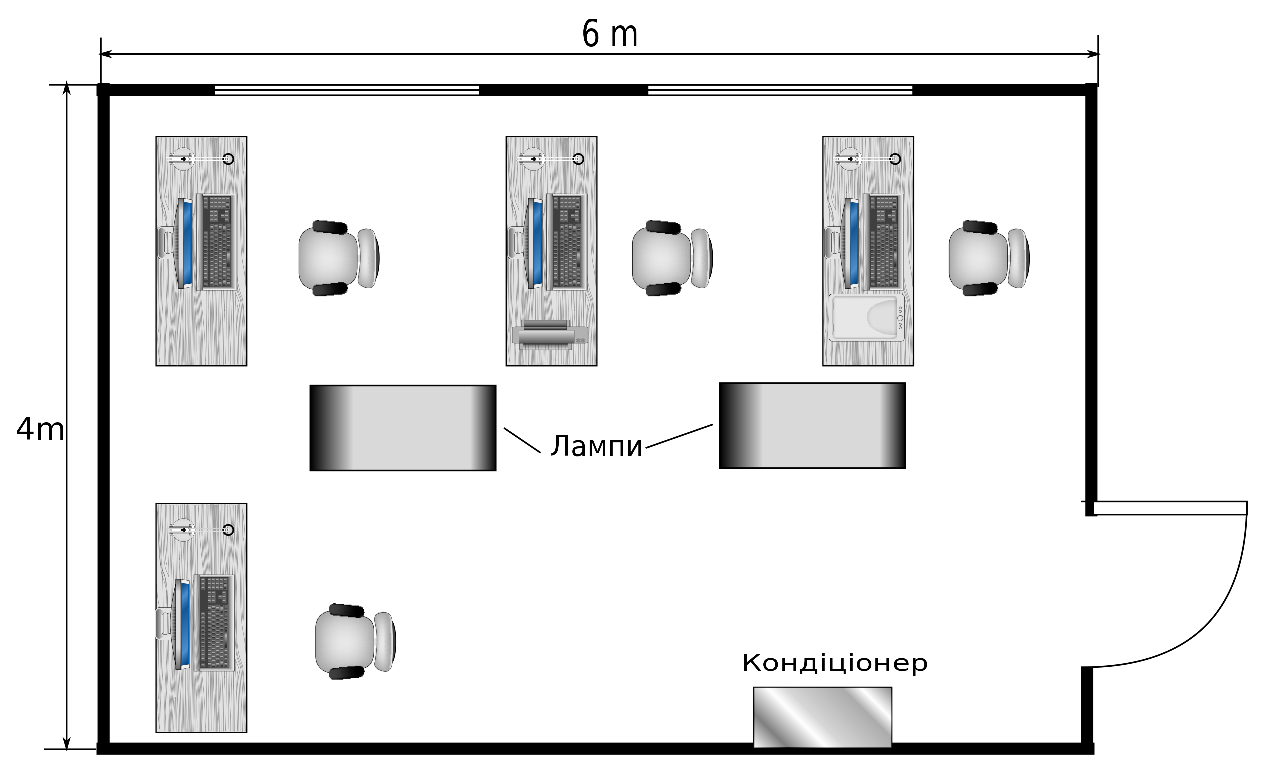
\includegraphics[width=\linewidth]{plan2.eps}
      \caption{План приміщення}
      \label{fig:plan}
    \end{figure}

    Санітарно"=гігієнічні вимоги щодо влаштування приміщень, в яких працівники
    працюють на персональних комп’ютерах, параметрів виробничого середовища,
    організації та обладнання робочих місць, режимів праці та відпочинку при
    роботі з відеотерміналами (ВДТ) і профілактичних медоглядів наведено
    у~\cite{npaop128}.

    Згідно з санітарними нормами з цього документу розмір площі для одного
    робочого місця оператора персонального комп’ютера повинен бути не менше
    $6.0$~м$^2$, а об’єм --- не менше $20.0$~м$^3$.
    Довжина кімнати --- $6.0$~м, ширина --- $4.0$~м, висота ---
    $2.7$~м.
    Маються також два вікна ($2.0$~м~$\times$~$1.6$~м), які спрямовані
    на північ.
    Отже, площа приміщення складає
      \[
        S = 6 \times 4 = 24~\text{м}^2,
      \]
    а обсяг
      \[
        V = 24 \times 2.7 = 64.8~\text{м}^2.
      \]
    Кожне робоче місце обладнане електронно"=обчислювальними машинами з
    РК"=моніторами Samsung LN32D403E2DXZA.
    У приміщенні постійно працює до чотирьох чоловік.
    Отже, на кожне робоче місце припадає по $6.0$~м$^2$ площі в об’ємі не
    менше, ніж $20.0$~м$^3$, що відповідає санітарним нормам.

    Санітарні норми також передбачають, що при розміщенні робочих столів з
    відеотерміналами слід дотримувати такі відстані: між бічними поверхнями
    ВДТ --- $1.2$~м, відстань від тильної поверхні одного відеотерміналу до
    екрана іншого відеотерміналу --- $2.5$~м.

    Параметри столу: довжина --- $1450$~мм, ширина --- $740$~мм, висота ---
    $730$~мм.
    Відстань між робочими столами також відповідає санітарним нормам, а саме
    не є меншою, ніж $2.0$~м.

    Робочі стільці є підйомно"=поворотні, регульовані за висотою, кутом нахилу
    сидіння та спинки.
    Поверхня сидіння --- плоска, а передній край --- заокруглений.
    Регулювання за кожним із параметрів здійснюється незалежно, легко та
    надійно фіксується.

    Екран ВДТ розташовується на відстані $670$~мм до очей користувача, що
    є оптимальною відстанню.
    Саме розташування екрану ВДТ забезпечує зручність зорового спостереження у
    вертикальній площині під кутом $30^\circ$.

    Столи були вибрані з урахуванням наступних умов:
    \begin{itemize}
      \item поверхня столу повинна володіти властивостями, що виключають появу
        відблисків в полі зору програміста;
      \item нижня частина столу повинна бути сконструйована так, щоб працівник
        міг зручно сидіти, не був вимушений підтискати ноги;
      \item висота столу повинна бути вибрана з урахуванням можливості сидіти
        вільно, в зручній позі, при необхідності спираючись на підлокітники;
      \item конструкція столу повинна передбачати наявність висувних ящиків.
    \end{itemize}

    Робоче приміщення, що розглядається, оснащене аптечками першої медичної
    допомоги.
    \clearpage
  \section{Аналіз шкідливих і небезпечних виробничих факторів}
    \subsection{Мікроклімат}
      Висока температура повітря негативно позначається на функціональному
      стані людини.
      Оптимальні та припустимі мікрокліматичні параметри у приміщеннях повинні
      враховувати специфіку технологічного процесу при використанні ПК.
      Зокрема, технічні умови експлуатації багатьох типів комп’ютерів містять
      допустимі робочі діапазони параметрів мікроклімату:
      \begin{itemize}
        \item температура повітря має знаходитись в межах від $10$ до
          $40^\circ C$;
        \item відносна вологість має знаходитися в межах від $40$ до $90\%$.
      \end{itemize}

      За даними ВООЗ, оптимальні значення температури у приміщенні становлять
      $19$--$23^\circ C$, відносна вологість повітря --- $55\%$, швидкість
      руху повітря не повинна перевищувати на рівні обличчя $0.1$~м/с.
      При відчутному нагрівання поверхонь (більше $45^\circ C$),
      контактуючих з людиною, передбачаються засоби охолодження або ізоляції.
      Особлива увага приділяється шляхом відводу повітря, щоб виключити
      перегрівання або протяг.

      Згідно з діючими в Україні нормативними документами\cite{dsn042} для
      даної категорії робіт (легка Iа) мають місце норми, наведені у
      табл.~\ref{tab:microclimat}.

      \begin{xtable}{|c|l|c|}{3}{Параметри мікроклімату для приміщень, де
        встановлені комп’ютери}{tab:microclimat}
          \hline
            Період року & Параметр мікроклімату & Величина\\
          \hline
            \multirow{3}{*}{Холодний} & Температура повітря & $22$--$24^\circ
            C$\\
          \cline{2-3}
            & Швидкість руху повітря & до $0.1$~м/с\\
          \cline{2-3}
            & Відносна вологість & $40$--$60\%$\\
          \hline
            \multirow{3}{*}{Теплий} & Температура повітря & $23$--$25^\circ
            C$\\
          \cline{2-3}
            & Швидкість руху повітря & $0.1$~м/с\\
          \cline{2-3}
            & Відносна вологість & $40$--$60\%$\\
          \hline
      \end{xtable}

      Завдяки встановленого кондиціонера можливо індивідуальне регулювання
      роздачі повітря в приміщенні.

      В процесі роботи змінюється концентрація іонів у повітрі робочої зони.
      Нормалізуючий вплив на аероіонний склад повітря робочої зони
      забезпечують: примусова вентиляція, захисні екрани та застосування
      іонізаторів.
      Повітря, що надходить у робочі приміщення, має бути очищене від
      забруднень, в тому числі від мікроорганізмів.

      Потужність (точніше, потужність охолодження) є основною характеристикою
      будь-якого кондиціонера.
      Серед різних моделей у нашому випадку пасує модель \texttt{RAS-30 CH1}
      фірми HITACHI, яка має потужність по холоду $4.14$~кВт.
      \clearpage
    \subsection{Шум}
      Встановлено, що шум погіршує умови праці, роблячи шкідливий вплив на
      організм людини.
      При тривалому впливі шуму на людину відбуваються небажані явища:
      знижується гострота зору, слуху, підвищується кров’яний тиск, знижується
      увага.
      Сильний тривалий шум може стати причиною функціональних змін
      серцево"=судинної і нервової систем.

      Нормативний рівень шуму не повинний перевищувати $50$~дБа\cite{dsn037}.

      У приміщенні маються внутрішні джерела постійного шуму: вентилятор
      блоків ПЕОМ ($35$~дБа, $8$~годин); принтери ($48$~дБа, $2$~години);
      дисковод ($40$~дБа, $0.5$~години).
      Зовнішніми джерелами шуму і вібрації в приміщенні є проїжджаючі
      транспортні засоби ($40$~дБа, $8$~годин).

      Отже, в приміщенні рівень шуму є допустимим, а отже засоби захисту не
      потрібні.
    \subsection{Освітлення}
      Природне світло проникає через бічні світло"=прорізи, зорієнтовані на
      північ, і забезпечує коефіцієнт природної освітленості (КПО) не нижче
      $1.5\%$.

      Як джерело світла при штучному освітленні повинні застосовуватися, як
      правило, люмінесцентні лампи типу ЛБ.
      У даному приміщенні застосовуються лампи NORTCLIFFE HF ECO з частотою
      перетворення $46$~кГц.
      Яскравість світильників загального освітлення в зоні кутів
      випромінювання від $50^\circ$ до $90^\circ$ відносно вертикалі в
      подовжній і поперечній площинах повинна складати не більше
      $200$~кд/м$^2$, а захисний кут світильників повинен бути не більшим за
      $40^\circ$.~\cite{dbn28}

      Рівень освітленості на робочому столі в зоні розташування документів має
      бути в межах $300$--$500$~лк.
      У разі неможливості забезпечити даний рівень освітленості системою
      загального освітлення допускається застосування світильників місцевого
      освітлення, але при цьому не повинно бути відблисків на поверхні екрана
      та збільшення освітленості екрану більше ніж до $300$~лк.

      Розраховуємо загальний світловий потік для освітлення площі робочого
      приміщення:
      \begin{equation}
        F_{n} = \frac{E_n S K_\text{зап} Z}{\eta},
        \label{eq:f-n}
      \end{equation}
      де $E_n$ --- нормоване значення штучної освітленості, $S$ --- площа
      приміщення, $K_\text{зап}$ --- коефіцієнт запасу, $Z$ --- коефіцієнт
      нерівномірності освітлення, $\eta$ --- коефіцієнт використання
      світильника.
      \[ F_{n} = (0.8 \times 24 \times 2 \times 1.5) / 0.55 = 1.2~\text{лм} \]

      Необхідна кількість світильників визначається за формулою:
      \begin{equation}
        n = \frac{F_n}{F_1},
        \label{eq:n}
      \end{equation}
      де, $F_n$ --- потрібний загальний світовий потік, $F_1$ --- світловий
      потік, створюваний одним світильником.
      \[ n = 1.2 / 0.5 = 2~\text{шт} \]
      \clearpage
    \subsection{Електробезпека}
      Згідно з Правилами улаштування електроустановок (ПУЕ, 2009~р.) дане
      приміщення відноситься до категорії приміщень без підвищеної безпеки.

      Електроживлення однофазне $220$~В з глухо"=заземленою нейтраллю,
      виконане 3-х провідних проводом.
      Для підключення обладнання встановлені розетки з заземлюючим контактом.
      Провідники заземлення приєднані до загального контуру заземлення.
      Опір загального становить $3$~Ом.
      Заземлення корпусів ЕОМ та іншого обладнання здійснюється через вилку
      підключення о джерела живлення.

      Дане робоче приміщення відповідає вимогам~\cite{dnaop131}.
    \subsection{Пожежна безпека}
      Дане приміщення відноситься до категорії B, класу П-IIа.
      До цієї зони відносяться приміщення, у яких використовуються тверді чи
      волокнисті речовини, нездатні переходити в зважений стан\cite{napb}.
      У приміщенні є пальні речовини: волокнисті(папір), тверді(дерево),
      пластмаси.

      Тому що ПЕОМ мають велику вартість, з огляду на категорію пожежної
      небезпеки приміщення, будинку з використанням ПЕОМ повинні бути I і II
      ступеня вогнестійкості (тобто всі конструктивні елементи повинні бути
      неспаленими).
      Фактично приміщення відповідає цим нормам (основні будівельні матеріали
      --- цегла, бетон, скло).

      У коридорах будинку установлюються пожежні крани.
      Вода використовується для гасіння пожеж у допоміжних службово"=побутових
      приміщеннях.
      Пожежні крани розташовують на висоті $1.35$~м від підлоги в найбільш
      доступних місцях.

      Для гасіння пожежі в початковій стадії його виникнення в приміщенні
      встановлено 2 вогнегасника: ВВ-5(з) (вогнегасник вуглекислотний закачний
      ємністю $1.3$~л.

      Для запобігання пожежі в приміщенні прийняті такі міри:
      \begin{itemize}
        \item передбачено вільний доступ до мережних рубильників і вимикачів;
        \item інструктаж з пожежної безпеки і періодичний контроль знань про
          правила пожежної безпеки;
        \item встановлені два димових сповіщувача ИПД-1;
        \item заборона використання електронагрівальних приладів;
        \item маються 2 вогнегасник ВВ-5(з);
        \item двері на шляху проходження людей відкриваються назовні;
        \item ширина загального коридору, ширина дверей, висота дверей
          відповідають нормативним значенням ОНТП 24-86;
        \item призначено відповідального за пожежну безпеку в приміщенні.
      \end{itemize}
      \clearpage
  \section{Інструкція з техніки безпеки}
    Дії працівників у разі виникнення пожежі:
    \begin{itemize}
      \item Про виникнення пожежі в приміщеннях негайно повідомити пожежну
        охорону за міським телефоном 101.
      \item При цьому необхідно назвати адресу, зазначити кількість поверхів
        будівлі, місце виникнення пожежі, обстановку на пожежі, наявність
        людей, а також повідомити своє прізвище.
      \item Вжити (по можливості) заходи на евакуацію людей, гасіння
        (локалізацію) пожежі з використанням первинних засобів пожежегасіння
        та на збереження матеріальних цінностей.
      \item Повідомити про виникнення пожежі керівника (заступників керівника)
        чи відповідальну компетентну посадову особу та чергового охорони.
      \item У разі необхідності, викликати інші аварійно"=рятувальні служби
        (медичну, газорятувальну тощо).
    \end{itemize}

\conclusion
  Метою даної роботи було дослідження та проектування системи відновлення
  змазуванняаних або розфокусованих зображень.
  В ході виконанні дипломної роботи були проаналізовані існуючі рішення для
  деконволюції, й порівняні їх обмеження.

  Під час огляду теоретичних відомостей були розглянуті такі поняття, як
  сигнал, одновимірний та багатовимірний; операція згортки, а також її варіант
  для двовимірного дискретного випадку; перетворення Фур’є.
  Було виявлено, що найкраще процес розфокусування й змазування описується
  через операції згортки.
  Були розглянуті основні види спотворень, що зустрічаються повсякденно:
  розмиття диском (боке), розмиття за Гаусом, змазування.
  Також були розглянуті методи зворотної згортки, деконволюції.

  Після вивчення теоретичного матеріалу, було проведене математичне
  моделювання, в ході котрого були порівняні методи, що були розглянуті під
  час вивчення теорії.
  Серед них слід зазначити метод інверсної фільтрації, самий швидкий з
  можливих методів.
  Але через те, що він не враховує наявність шуму в зображенні, перевагу було
  надано іншим методам: методу Люсі"=Річардсона та фільтру Вінера.
  Фільтр Вінера використовує дещо складніший математичний апарат, проте працює
  значно швидше, ніж метод Люсі"=Річардсона.

  Також під час математичного моделювання було досліджено те, наскільки якісно
  ці методи дозволяють відновити зображення після того чи іншого спотворення.
  Методи Люсі"=Річардсона та Вінеру дозволяють отримати результати майже
  однакової якості для всіх типів розмиття, проте фільтр Вінеру значно
  швидший.
  Саме через це для програмної реалізації та подальшого тестування був обраний
  цей алгоритм.

  Оскільки фільтр Вінера є методом несліпої деконволюції, для коректної роботи
  алгоритму необхідно вказати деяке наближення функції розподілу точки.
  Через це було проаналізовано та змодельоване метод отримання деякого
  наближення функції спотворення.
  На прикладі реальних зображень, що були збережені з певним розмиттям, було
  знайдено деяке наближення до функції розподілу точки таке, що відновлені
  зображення були значно кращими по якості за вхідні.

  Було розроблено програмний модуль, що дозволяє безпосередньо відновлювати
  зображення у автоматизованому режимі: користувачу потрібно лише вказати
  необхідний, елементарний тип розмиття та дещо корегувати його параметри.
  Отриманий програмний засіб є досить швидкодіючим у порівнянні з комерційними
  аналогами.

  Для подальшого розвитку слід зазначити можливість дослідження методів сліпою
  деконволюції, а саме критеріїв якості зображення та критеріїв корегування
  функції розподілу точки.
  Впровадження цієї методики проводити відновлення фотографій без дій
  користувача в автоматичному режимі.
  Також слід зазначити, що потрібно розглянути можливість декомпозиції
  складної функції розподілу точки на менш складні складові.
  \clearpage
\begin{thebibliography}
  \bibitem{deconvolve-index} P.J. Tadrous Deconvolve.net / P.J. Tadrous
  \bibitem{richardson-hadley} Richardson, William Hadley Bayesian-Based
    Iterative Method of Image Restoration, 1972
  \bibitem{book2} A.P. Demster, N.M. Laird, D.B. Rubin Maximum Likelihood from
    Incomplete Data via the EM ALgorithm / J. Royal Stat. Soc. Ser. B, 1977
  \bibitem{npaop128} НПАОП 0.00-1.28-10 <<Правила охорони працi пiд час
    експлуатацiї електронно"=обчислювальних машин>>. --- 26 березня 2010 р.
  \bibitem{dnaop131} ДНАОП 0.00-1.31-99 <<Правила охорони працi пiд час
    експлуатацiї електронно"=обчислювальних машин>>. --- 17 червня 1999 року.
  \bibitem{dsn042} ДСН 3.3.6.042-99. <<Санiтарнi норми мiкроклiмату виробничих
    примiщень>>. --- 01 грудня 1999 р.
  \bibitem{dsn037} ДСН 3.3.6.037-99. <<Державнi санiтарнi норми виробничого
    шуму, ультразвуку та iнфразвуку>>. --- 2000.
  \bibitem{napb} НАПБ А.01.001-2004. Правила пожежної безпеки в Українi. ---
    2004.
  \bibitem{honsales-woods} Гонсалес Р., Вудс Р. Цифровая обработка изображений
  \bibitem{honsales-woods-eddins} Гонсалес Р., Вудс Р., Эддинс С. Цифровая
  обработка изображений в среде MATLAB.
  \bibitem{dbn28} ДБН В.2.5-28-2006. <<Природне та штучне освiтлення>>. ---
  2006.
  \bibitem{knuth} D. Knuth. Seminumerical Algorithms (3rd.\ ed.) /
  Addison–Wesley, 1997 --- ISBN 0-201-89684-2.
  \bibitem{wiener} N. Wiener. Extrapolation, Interpolation, and Smoothing of
  Stationary Time Series / MIT Press, 1964 --- ISBN 0-262-73005-7
  \bibitem{numerical} W. Press, S. Teukolsky, W. Vetterling, B. Flannery.
  Numerical Recipes 3rd Edition: The Art of Scientific Computing / Cambridge
  University Press, 2007


\end{thebibliography}
\append{1}{Вихідні тексти на мові Matlab}
      \lstinputlisting{show-fft.m}
      \clearpage
      \lstinputlisting{blurred-invfilter.m}
      \clearpage
      \lstinputlisting{test-methods.m}
      \clearpage
\append{2}{Вихідні тексти на мові C++}
\lstset{language=C++}
  \lstinputlisting{smartDeconv/src/DeconvolutionTool.h}
      \clearpage
  \lstinputlisting{smartDeconv/src/ImageUtils.h}
      \clearpage
% \clearpage
% \bibliographystyle{ugost2008ls}
% \bibliography{src}
\end{document}
